\documentclass[twocolumn, 9pt,fleqn]{jsproceedings}

\interfootnotelinepenalty=10000

\renewcommand\refname{References}

\title{Visual Localization for Autonomous Navigation}

\author{Helio Perroni Filho (Doctorate Course, 2nd year)\authorrefmark{1}}

\affiliation{Intelligent Robotics Laboratory, OHYA's group}

\abstract{
Differential Visual Streams (DiVS) is an image processing method to compare sequences of landscape images captured by an approaching observer. It works on monocular images recorded by a single uncalibrated camera. Experiments show DiVS provides a sound basis for an appearance-based navigation system able to work both indoors and outdoors, against variations in lighting and landscape composition.
}

\keywords{Image Processing, Machine Learning, Navigation}

\begin{document}
\thispagestyle{myheadings}
\markright{2014年度 第3回 山彦シンポジウム [2015/02/19--02/21 国立オリンピック記念青少年総合センター]}
\maketitle

\authorreftext{1}{Graduate School of Systems and Information Engineering,\\ University of Tsukuba}

\section{Introduction}

Autonomous navigation is a central topic in mobile robotics, with a variety of useful applications~\cite{BON02,ARK90}. One recurrent use case is \textit{teach-replay}, where a robot guided through an environment once (the teaching step) must later autonomously retrace the original path (the replay step)~\cite{BUR01}. In the absence of measurement errors, this could be easily achieved by recording odometry data. In practice, however, any intrinsic localization method is subject to \textit{drift}, the unrecoverable buildup of reading errors. Figure~\ref{fig:drift} illustrates the problem.

\begin{figure}[h!]
\vspace{20pt}
\includegraphics[width=\columnwidth]{drift.pdf}
\vspace{10pt}
\caption{Runway drift in odometry-based navigation systems. As the robot moves, its pose $(x, y, \theta)$ as reported by odometry (the dashed line) increasingly diverges from the actual pose $(x', y', \theta')$ (the solid line).}
\label{fig:drift}
\end{figure}

Solutions to the drift problem usually involve leveraging distinct environment features, otherwise known as \textit{landmarks}, as reference points relative to which the robot can more reliably locate itself. The problem then becomes how to detect effective landmarks, and how to describe the relation between landmark readings and robot position. Methods proposed over the years can be roughly divided into \textit{map-based} and \textit{mapless}, according to whether they rely on representations of the environment's structure; map-based methods can be further divided in \textit{metric}, where the environment is represented as a metric grid in 2D or 3D space, and \textit{graph-based}, where a graph representing specific locations as nodes and relations of reachability as edges is used instead~\cite{BON02}.

Simultaneous Localization and Mapping (SLAM) is a popular metric map-based approach. Initially supported mainly by range sensors such as laser and ultrasound, recent advances and wider hardware availability have increased the number of such systems that employ cameras as navigation sensors~\cite{DAV07,CUM08}. Unfortunately, the need to keep an accurate map, and precisely track the robot's pose within it, have always placed an upper bound on the geographic reach of SLAM systems~\cite{CAS04}.

The complexity and limitations of map-based navigation systems have motivated work in graph-based navigation methods, particularly \textit{appearance-based navigation}. In this paradigm the environment is represented as image sequences collected along a route; such snapshots are matched against live sensory input in order to estimate current robot pose~\cite{BON02}. Compared to map-based approaches, it constitutes a less computationally expensive, more intuitive model, closer to how humans navigate our surroundings. The typical appearance-based navigation use case is \textit{teach-replay}, where a robot is led through an environment by a guide (the teach step), and must then autonomously retrace the original path, orienting itself by the data gathered during the guided phase (the replay step)~\cite{BUR01}.

This article presents \textit{Differential Visual Streams} (DiVS), an image processing method for matching image sequences captured over the same environment under varying conditions. Remaining sections are organized as follows: first, related works are presented in terms of core methods, sources of input, test environments and variations allowed between teach and replay steps. It is shown there is a lack of systems that work both indoors and outdoors, under varying environmental conditions, and restricted to off-the-shelf hardware. DiVS is then described, and experiments are reported, demonstrating the method's resilience under a range of environmental variations, both indoors and outdoors. Directions for further research are discussed in the conclusion.

\begin{table}[t]
\centering
\caption{Summary of appearance-based navigation methods proposed in the literature, characterized in terms of employed sensors, test environments, and variations allowed between teach and replay steps.}
\renewcommand{\arraystretch}{1.5}
\setlength{\tabcolsep}{5pt}
\tiny
\begin{tabular}{|m{2.2cm}|m{1.4cm}|m{0.7cm}|c|c|c|}
\hline
    \multirow{2}{*}{\centering Method} & \multirow{2}{*}{Sensors} & \multirow{2}{*}{Tested} & \multicolumn{3}{|c|}{Landscape Variations} \\
\cline{4-6}
    & & & Lighting & Occlusion & Movement \\
\hline
    \mbox{Minimal template matching} \mbox{error~\cite{MAT96}} & Monocular camera & Indoors & No & No & No \\
\hline
    \mbox{Cost function} \mbox{minimization~\cite{OYA96}} & Monocular camera & Indoors & No & No & No \\
\hline
    \mbox{Mutual information~\cite{STE12}} & Monocular camera & Indoors & No & Yes & Yes \\
\hline
    Feature point tracking~\cite{CHE06} & Monocular camera & Indoors, Outdoors & Yes & No & Yes \\
\hline
    \mbox{Local best match and} \mbox{sequence recognition~\cite{MIL12}} & Monocular camera & Outdoors & Yes & Yes & Yes \\
\hline
    \mbox{Stereo feature matching and} \mbox{visual motion estimation~\cite{KIM08}} & Stereo camera & Indoors & Yes & Yes & Yes \\
\hline
    Average Landmark Vector~\cite{LAM00} & $360^o$ panoramic camera, polarized light sensor, wheel encoders & Simulation, Outdoors & Yes & No & No \\
\hline
    \mbox{Block matching} \mbox{Optical Flow~\cite{VAR05}} & $360^o$ panoramic camera, wheel encoders & Indoors & Yes & Yes & No \\
\hline
\end{tabular}
\label{tab:methods}
\end{table}

\section{Related Work}

Appearance-based navigation methods built on cost minimization define a mismatch metric between any two images, then pair up replay images to least mismatched teach images. The remaining mismatch can then be analyzed to provide an estimate of the displacement between corresponding viewpoints. Template matching~\cite{MAT96} is an intuitive choice of mismatching metric: the quality of the match can be used to pair current input to stored images, and the image coordinates of the best match provide a first approximation of pose displacement. A more involved alternative, noted for its resource efficiency~\cite{BON02} is to extract vertical lines from teach and replay images, then define mismatch in terms of differences in intensity, position and number of lines in each set~\cite{OYA96}. However, these metrics are vulnerable to changes in lighting, landscape appearance and the presence of moving objects, having been successfully tested only in static indoors environments. Mismatch metrics in general are also susceptible to ambiguities in environments with many repeating features, such as long corridors.

Mutual information~\cite{STE12} and Kanade-Lucas-Tomasi (KLT) feature tracking~\cite{CHE06} have been proposed as more robust mismatch metrics. Ambiguities over repeating environmental features can be resolved by splitting teach records in segments delimited by milestone frames, and then limiting the search to a single segment at a time. The transition from one segment to the next can be determined by watching the intensity of the mismatch between current input and the next milestone: a reversal from a decreasing to an increasing trend indicates the milestone has been passed~\cite{MAT96,CHE06}.

Another way to make mismatch minimization more robust is to look not for a global best match for each visual input, but instead to look for coherent sequences of ``good'' matches between successive replay inputs and the teach record~\cite{MIL12}. Tested on video clips recorded from manually driven cars, this method was highly successful in recognizing revisited locations over a wide range of variations (day, night, rain, moving cars, seasonal changes, etc), but no tests involving actual autonomous navigation were performed, and test landscapes were restricted to open outdoors spaces.

Stereo vision systems can also use the KLT tracker to find correspondences between feature points in three-dimensional space. This method is less vulnerable to ambiguities in appearance, though it must still be complemented by motion estimation for cases where feature matching is not possible (e.g. due to the presence of moving elements or changes to the landscape)~\cite{KIM08}. This method was shown to reliably retrace paths as long as $60m$, but no results on lighting changes or outdoor tests have been reported.

Finally, panoramic cameras make possible to use methods that compare current visual input and stored images to compute \textit{direction vectors} pointing towards a target pose~\cite{LAM00,VAR05}. In this way the need for image pairing is sidestepped, as direction vectors make possible to directly locate the current pose relative to all known records. However those methods require that a common landmark set remain visible throughout both teach and replay steps, limiting applicable range as well as robustness to landscape changes. Additionally, ensuring the panoramic camera will have a clear field of view all around the robot might be problematic from an engineering perspective, depending on form-factor considerations and application scenarios.

\section{Method}

DiVS works on a pair of image streams: a prerecorded \textit{teach stream} depicting a desired travel across a target environment, and a \textit{replay stream} of a subsequent attempt to retrace the original travel. For a mobile robot relying on DiVS to provide steering guidance, the replay stream will be a real-time video feed, but for testing purposes it might as well be prerecorded too.

DiVS is composed of three stages: difference stream computation, image pairing, and shift estimation. The next subsections will describe each step in detail.

\subsection{Difference Streams}

Given an \textit{image stream}, i.e. a sequence of snapshots collected over time, the \textit{image stream function} $S(k) = I_k$ returns the $k^{th}$ recorded image $I^{m \times n}$ of the field of view. Obviously, as the stream's source moves about the environment, the contents of each $I_k$ will vary accordingly. Such changes can be quantified by a \textit{difference image} function of short-term changes to the visual input:
\begin{equation}
D(k, \delta) = | S(k) - S(k + \delta) |
\end{equation}

Where the subtraction operator is defined for images as pixel-wise subtraction (equivalent to how matrix subtraction is defined as cell-wise subtraction), and the parameter $\delta > 0$ specifies a gap between compared images.

Difference images have useful properties for scene recognition. Assuming an appropriate gap for the stream's pace of change, each difference image should contain regions of high difference (corresponding to the apparent movement of image discontinuities such as edges) and others significantly lower (corresponding to the inside of object surfaces); moreover, discontinuities related to close-by objects generate larger differences than those pertaining to farther removed ones. This allows a glimpse into the scene's structure, which can be explored to enable robust scene classification. Finally, absent of saturation artifacts, difference images are largely invariant to ambient brightness, providing a degree of normalization across illumination conditions.

However, defining an appropriate frame gap for difference image computation is not a trivial task. Too short a gap will result in a mostly empty image; too large and it may become impossible to relate differences to actual scene elements. The ideal value will likely change continuously over the length of a given image stream, depending on factors such as the stream source's speed, its direction of movement, and the environment's composition. Therefore, in order to ensure the quality of difference images remains roughly constant, a \textit{sampling strategy} $p(k, \tau)$ is defined such that:
\begin{equation}
p(0, \tau) = 0
\end{equation}
\begin{equation}
p(k, \tau) = k + \arg \min_{\delta} \; \langle D(p(k - 1, \tau), \delta) \rangle \geq \tau
\end{equation}

Where $\langle \cdot \rangle$ is the average operator and $\tau$ a threshold average difference. Combining the image stream function and the sampling strategy above it's possible to define the \textit{Difference Stream} function $DiS(k, \tau) = J_k$ such that:
\begin{equation}
DiS(k, \tau) = | S(p(k, \tau)) - S(p(k - 1, \tau)) |
\end{equation}

Figure~\ref{fig:dis} illustrates the process.

The use of the sampling strategy $p(k, \tau)$ in the definition of $DiS(k, \tau)$ ensures that each difference image approximates the optimal average difference $\tau$. This provides a degree of consistency across the stream, even in the face of changes to physical parameters such as the stream source's speed and direction of movement.

\subsection{Image Pairing}

Appearance-based navigation methods commonly require pairing up teach and replay images by viewpoint proximity. Formally, let the image streams for a prerecorded teach step and ongoing replay step be represented respectively by:
\begin{alignat}{3}
& S_{teach} & = & [I_1, \dotsc, I_i, \dotsc, I_m] \\
& S_{replay} & = & [I'_1, \dotsc, I'_j, \dotsc, I'_n]
\end{alignat}

The robot's pose at the instant an image $I$ was taken is given by the \textit{viewpoint function}:
\begin{equation}
o(I) = (x, y, \theta)
\end{equation}

The \textit{pairing function} $g(I'_j)$ is defined over the domain of replay step images such that  $g(I'_j) = I_i$ is the teach image whose corresponding viewpoint $o(I_i)$ is the most similar to the viewpoint $o(I'_j)$ of replay image $I'_j$:
\begin{equation}
g(I'_j) = \arg \min_{I_i \in S_{teach}} {\|o(I_i) - o(I'_j)\|}
\end{equation}

\begin{figure}[t]
\includegraphics[width=\columnwidth]{dis.pdf}
\caption{Difference stream computation. Given an image stream $S$ (a), pairs of images are selected according to sampling strategy $p(k, \tau)$ (b) and subtracted (c), producing the images of the difference stream (d).}
\label{fig:dis}
\end{figure}

Obviously if $o(I)$ were reliably known at any one time there would be no need for image pairing in the first place. Therefore what is needed is an approximation $g'(I'_j)$ that circumvents this requirement. In particular, \textit{appearance-based pairing} methods exploit the insight that changes to robot pose cause predictable changes to visual input, and therefore it must be possible to design an image similarity metric that correlates well to pose proximity~\cite{HEL13b}. Difference images are robust to environmental variations and tend to emphasize elements that stand out relative to its surroundings, making difference streams a convenient domain over which to implement appearance-based pairing.

Given difference streams $DiS_{teach}(i, \tau)$ and $DiS_{replay}(j, \tau)$ from the teach and replay steps respectively, let the \textit{stream window} functions $Z_{teach}(t)$ and $Z_{replay}(t)$ be defined as:
\begin{alignat}{3}
& Z_{teach}(t) & = & [J_i \; | \; J_i = DiS_{teach}(i, \tau) \; , \; t - z \leq i < t] \\
& Z_{replay}(t) & = & [J'_j \; | \; J'_j = DiS_{replay}(j, \tau) \; , \; t - z \leq j < t]
\end{alignat}

Initially let $t = z$. From each replay difference image a list of \textit{attention points} is extracted by selecting points of maximum intensity within a neighborhood of length $\alpha$:
\begin{equation}
P(J'_j) = [p_{j,k} \; | \; J'_j[p_{j,k}] \geq J'_j[p_{j,k} - \alpha : p_{j,k} + \alpha ]]
\end{equation}

Where $p_{j,k} = (u, v)$ is a point in image coordinates. Attention points determine locations over the field of view for comparison between a replay difference image and difference images from the teach sequence. However individual points are unlikely to provide enough similarity information, therefore whole regions surrounding attention points must be extracted for comparison. Given a attention point $p_{j,k}$, a difference image $J$ (not necessarily related to $p_{j,k}$ in any way) and a \textit{padding} $d$, a \textit{patch} $C(p_{j,k}, J, d)$ is defined as a square section of side $2w+1$ taken from difference image $J$ around $p_{j,k}$:
\begin{equation}
C(p_{j,k}, J, d) = J[p_{j,k} - d : p_{j,k} + d]
\end{equation}

For each attention point, a patch of padding $\alpha$ is extracted from its originating replay image, and one patch of padding $\beta$ (such that $\alpha < \beta$) is extracted from each teach difference image. The \textit{response} generated by a replay patch relative to a teach patch is defined as:
\begin{equation}
r(i, j, k, \alpha, \beta) = \max \big( C(p_{j,k}, J_i, \beta) \star C(p_{j,k}, J'_j, \alpha) \big)
\end{equation}

Where $\star$ is the normalized cross-correlation operator~\cite{HEL14b}. The response provides a measure of how much images $J_i$ and $J'_j$ ``look like'' each other in the neighborhood of attention point $p_{j,k}$, given that a limited degree of sliding of $J'_j$ over $J_i$ is allowed.

The \textit{local best match} $b(j, k, \alpha, \beta) = i \in [1, n]$ is the index of the teach difference image that produces the best response for a given replay difference image $J'_j$ and attention point $p_{j,k}$ subject to paddings $\alpha$ and $\beta$, that is:
\begin{equation}
b(j, k, \alpha, \beta) = \arg \max_{i \in [1, m]} {r(i, j, k, \alpha, \beta)}
\end{equation}

The \textit{similarity} $l(i, j, \alpha, \beta)$ between $J_i$ and $J'_j$ can then be defined as the number of attention points extracted from $J'_j$ whose local best matches are found on  $J_i$, that is:
\begin{equation}
l(i, j, \alpha, \beta) = \sum_{k = 1}^{z} {
\left\{
\begin{array}{r r}
1 & \text{if } b(j, k, \alpha, \beta) = i \\
0 & \text{otherwise}
\end{array}
\right.
}
\end{equation}

Because replay patches are allowed to ``slide'' over the larger teach patches to find a good match, and a relative majority of correct matches can ``vote out'' mistaken ones, this definition of similarity is robust against limited viewpoint variations and landscape changes. However it is still possible to get poor pairings, especially when there is not a clear consensus among local best matches. Results can be improved by exploiting the monotonic nature of the pairing function -- image indexes must always increase, at a rate roughly proportional to the stream source's speed at the time it was recorded.

A \textit{similarity map} $\Gamma_{\alpha,\beta}$ is a $z \times z$ matrix such that:
\begin{equation}
\Gamma^{\; z \times z}_{\alpha,\beta} = [\gamma_{\; i,j} = l(i, j, \alpha, \beta) \; | \; i \in [1, z] \; , \; j \in [1, z]]
\end{equation}

In a similarity map, high similarity values tend to gather in roughly diagonal clusters: this is the direction along which both teach and replay difference image indexes increase. A diagonal line can be fit over such clusters by solving the following optimization problem:
\begin{equation}
\begin{aligned}
& \underset{i_1, j_1, i_u, j_v}{\text{maximize}}
& & L(i_1, j_1, i_u, j_v) = \sum_{j = j_1}^{j_v}{\Gamma_{\alpha,\beta}[j \frac{i_u - i_1}{j_v - j_1}, j]} \\
& \text{subject to}
& & i_1 = 1 \text{ or } j_1 = 1 \\
&
& & i_u = m \text{ or } j_v = z
\end{aligned}
\end{equation}

This problem can be solved efficiently by following the steps below:

\begin{enumerate}
\item Calculate the Hough Transform~\cite{DUD72} of the similarity maps with parameters $\rho = 1$ and $\theta = 1^o$, generating the list \mbox{$L = [f_1, \dotsc, f_l, \dotsc, f_w]$} such that $f_l(x) = y$ is a line in $\mathbb{Z}^2$;
\item Generate the sublist $L' \subseteq L$ by discarding any non-increasing lines, i.e. lines where $f(x_1) \geq f(x_2) \; | \; x_1 < x_2$;
\item For each remaining line $f'_l \in L' \; | \; f'_l(x) = y$, compute the quality function $\psi(f) = \sum_{x = 0}^{m} \Gamma[f(x), x]$;
\item Select the line of maximum quality:
\begin{equation}
f_b = \arg \max_{f' \in L'} {\psi(f')} \notag
\end{equation}
\item If $f_b(1) \geq 1$ then make $j_1 = 1$ and $i_1 = f_b(1)$, otherwise make $i_1 = 1$ and solve $f_b(j_1) = 1$ to find $j_1$;
\item If $f_b(z) \leq m$ then make $j_v = z$ and $i_u = f_b(z)$, otherwise make $i_u = m$ and solve $f_b(j_v) = m$ to find $j_v$.
\end{enumerate}

An initial approximation of the pairing function can then be defined as:
\begin{equation}
g'(I'_j) = I_i \; | \; i = j \frac{i_u - i_1}{j_v - j_1}
\end{equation}

Image pairs beyond the initial $z \times z$ set of teach and replay difference images can be found by repeating the process above for $t = z + 1$, $t = z + 2$ etc. and computing $g'(I'_t)$.

\subsection{Shift Estimation}

After being paired up, teach and replay difference images can be compared in terms of \textit{shift}, the apparent differences in the position of landmarks (or rather, the traces they left) in one difference image relative to the other. Given two difference streams $A$ and $B$, if $A$ was recorded in a path ``to the left'' of the path that originated $B$, it is expected that each difference image $J_{A,k}$ will be ``right-shifted'' relative to a corresponding $J_{B,k'}$ -- that is, features from $B$ will be consistently found in $A$, but in positions further to the right. Therefore, the shift between difference images is a proxy to the physical drift experienced by the robot recording the image sequences used to compute them. Furthermore, mobile robots are generally assumed to drive across flat surfaces, and in this context shift can be reduced to a 1D problem space -- difference images can shift ``left'' or ``right'', but not ``up'' or ``down''. Accordingly, it would be convenient to have a 1D representation of shift that allowed quick estimation of sideways drift.

A procedure for calculating such a 1D representation can be defined as follows. Given a pair $(J_i, J'_j)$ of difference images from the teach and replay streams respectively, the first step is to split them vertically across the middle and discard the lower halves, generating the difference half-images $(U_i, U'_j)$. This is done because of the poor signal-to-noise ratio in the lower half of difference images: they mostly depict the environment's floor, which is at best largely empty, and at worst filled by traces of repeating elements such as the edges of floor tiles.

Next $U_i$ is split in $e$ slices of equal width, and each slice is correlated to $U'_j$ using a normalized variation of the Fourier cross-correlation method~\cite{HEL14b}. For each slice of $U_i$ a \textit{shift vector} $V(k, e, U_i, U'_j)$ is computed as the first line of the correlation map between itself and $U'_j$:
\begin{equation}
V(k, e, U_i, U'_j) = (U'_j \star U_i[:, k*e:(k+1)*e])[0,:]
\end{equation}

The shift vectors for each slice of $U_i$ are computed and summed up by the $SHIFTS(e, U_i, U'_j) = F_j$ function defined as:
\begin{equation}
SHIFTS(e, U_i, U'_j) = \sum_{k=0}^{\frac{n}{e}}{(\hat{0}^n \; \| \; V(k, e, U_i, U'_j) \ll k*e}
\end{equation}

Where $\hat{0}^n$ is the zero vector of dimension $n$, and the concatenation operator $\|$ is defined for any two vectors $a = (a_1, \dotsc, a_m)$ and $b = (b_1, \dotsc, b_n)$ such that $a \; \| \; b = (a_1, \dotsc, a_m, b_1, \dotsc, b_n)$.

In procedural terms, $SHIFTS(e, U_i, U'_j)$ places a window of width $e$ over $U_i$, then calculates the normalized cross-correlation of $U'_j$ by the contents of the window. The window is then slided $e$ positions to the right, and the operation repeated. At every step a new shift vector of length $n$ is computed. The $n / e$ vectors must then be summed to produce a final shift estimation, but first one issue has to be addressed.

\begin{figure}[t]
\includegraphics[width=\columnwidth]{slide_cc.pdf}
\caption{Shift vector computation. A replay difference image (a) is repeatedly cross-correlated with the contents of a window of width $e$ sliding across the corresponding teach difference image (b), producing at every turn a cross-correlation vector of same length (c). The $n / e$ cross-correlation vectors are zero-padded from the left to length $2n$ (gray squares indicate padding cells), left-shifted by $ke$ pixels (i.e. the position of the window when they were calculated), and summed (d). The resulting \textit{shift vector} describes the likelihood of different degrees and directions of shift (e).}
\label{fig:slide_cc}
\end{figure}

Each shift vector measures the similarity between $U'_j$ and a different slice of $U_i$. For a section taken from a initial position $k > 1$, coefficients from positions prior to $k$ indicate the likelihood of a left shift, and positions following, of a right shift. For example, the first vector, which was produced when the sliding window was at position $k = 0$, can only ever indicate shifts to the right. The next one, however, computed when the window was on position $k = 1$, can conceivably report a shift of at most one position to the left, and as many as $n-1$ positions to the right. In order words, shift vectors are anchored to different origin points relative to $U'_j$. To account for this, each vector is zero-padded from the left to length $2n$, then left-shifted $k*e$ positions -- i.e. the position of the window when they were calculated. Figure~\ref{fig:slide_cc} illustrates the process.

\begin{figure}[h!]
\subfloat[Raw shift map]{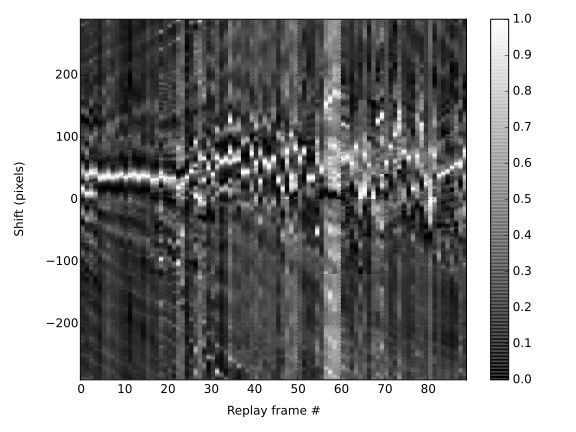
\includegraphics[width=\columnwidth]{selection_0.pdf}}\\
\subfloat[Averaged shift map]{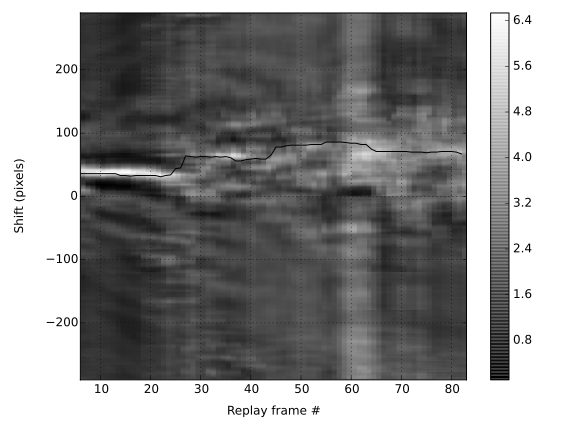
\includegraphics[width=\columnwidth]{selection_6.pdf}}
\caption{Raw shift map (a) and average over 6 vectors (b). Contour maps show shift likelihood across a sequence of shift vectors. Horizontal axis is replay image index, while vertical axis is image shift $p$ in pixels. Brighter points indicate higher likelihood. Values at $p_0 = 0$ indicate the likelihood of no shift, values at $p_l > 0$ indicates likelihood of left shift by $p_l$ pixels, and $p_r < 0$, of right shift by $|p_r|$ pixels. Starting from a global maximum estimate, hill climbing is performed on the smoothed shift map (b) to update the selected shift while avoiding too much of a deviation from previous values.}
\label{fig:selection}
\end{figure}

After summing the padded and shifted vectors, the resulting shift vector is a map of shift likelihoods: the central value indicates the likelihood that no shift has taken place, while values prior to it represent the likelihood of a shift to the left, and values following, of a shift to the right. Shift vectors are generally consistent over extended ranges, but abrupt changes are sometimes observed, especially if there are differences in landscape composition (e.g. presence / absence of moving elements) between test and replay streams. Such occasional mismatches can be averaged out by computing \textit{averaged shift vectors} such that:
\begin{equation}
\overline{F^w_k} = \frac{1}{w} \sum_{i=1}^{w}{F_{k-i}}
\end{equation}

All that is left is to select a definite output from the shift vector. It's possible to simply select the position of maximum coefficient at every turn, but this might result in shift estimates changing abruptly over time. To make estimates more smooth, the last $w$ individual shift vectors are averaged, and iterative hill climbing is performed over successive averaged shift vectors. Figure~\ref{fig:selection} illustrates shift vector averaging and hill-climbing shift selection.

\section{Experiments}

Two test environments were selected in the campus of the University of Tsukuba, henceforth referred to as ``indoors'' and ``outdoors'': the corridor in front of laboratory room 3D402 (the ``indoors'' environment) and the paved way by the side of faculty building 3D (the ``outdoors'' environment). The indoors environment featured a smooth floor; the outdoors environment's floor, while basically flat, was rough enough to add a noticeable amount of vibration to robot movement. Trips of $20m$ of length were recorded in the indoors environment; in the outdoors environment, in order to avoid reaching a patch of excessively rough terrain, trip lengths were reduced to $15m$.

\begin{figure}[t]
\centering
\subfloat[Indoors teach example]{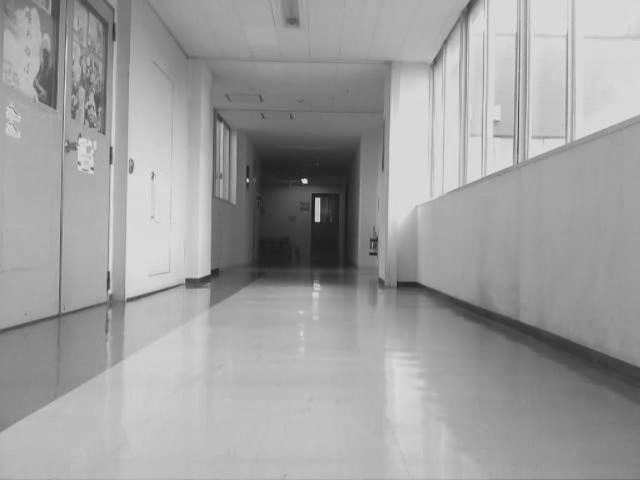
\includegraphics[width=0.4\columnwidth]{indoors_teach.eps}}%
\hspace{0.1\columnwidth}%
\subfloat[Indoors replay example]{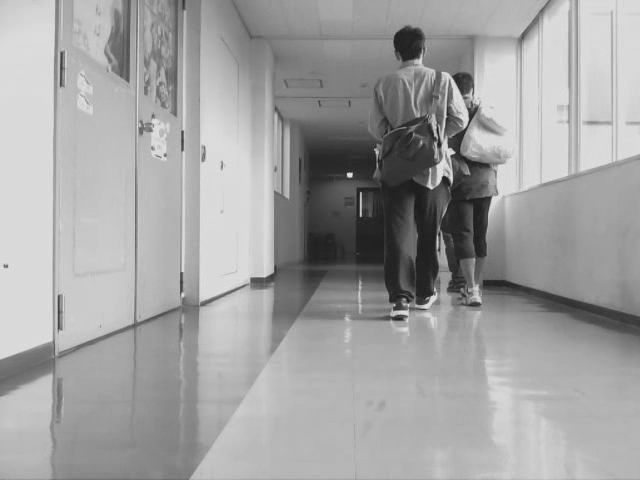
\includegraphics[width=0.4\columnwidth]{indoors_replay.eps}}\\
\subfloat[Outdoors teach example]{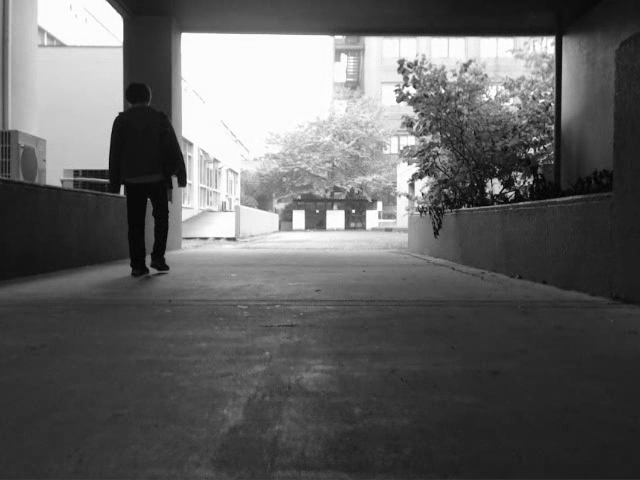
\includegraphics[width=0.4\columnwidth]{outdoors_teach.eps}}%
\hspace{0.1\columnwidth}%
\subfloat[Outdoors replay example]{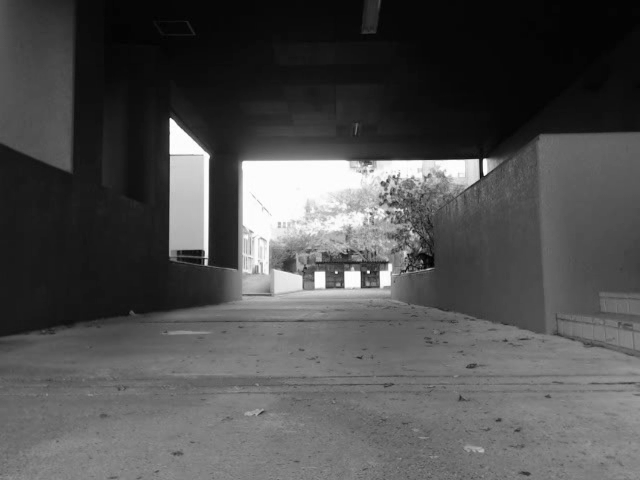
\includegraphics[width=0.4\columnwidth]{outdoors_replay.eps}}
\caption{Image samples from the indoors teach (a) and replay (b) step sequences, as well as outdoors teach (c) and one of the replay (d) step sequences. Between $30s$ and $50s$ into the indoors replay step three people came from behind the robot, staying on the right side of the field of view as they walked away; likewise, in the outdoors teach step a pedestrian came from behind the robot, staying on the left side of the visual field as he walked away from $20s$ to $40s$.}
\label{fig:environments}
\end{figure}

\begin{figure}[h]
\centering
\subfloat[Mismatched images]{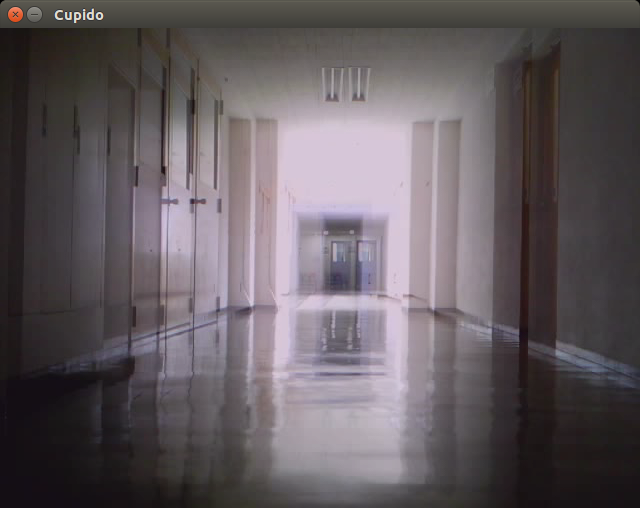
\includegraphics[width=0.4\columnwidth]{cupido_01.eps}}%
\hspace{0.1\columnwidth}%
\subfloat[Perfect match]{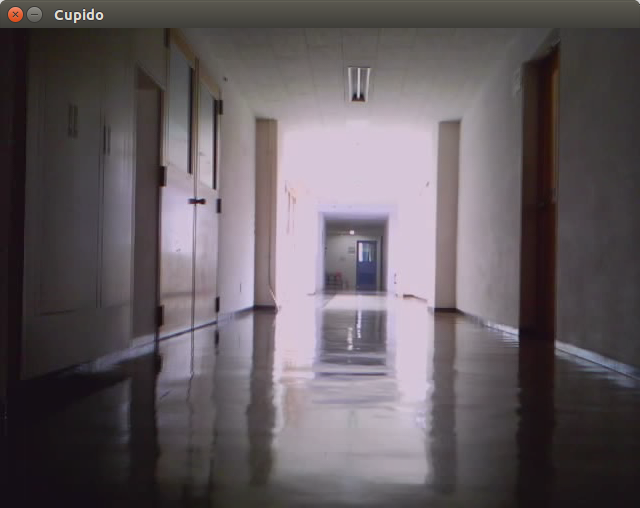
\includegraphics[width=0.4\columnwidth]{cupido_02.eps}}\\
\subfloat[Matching far features]{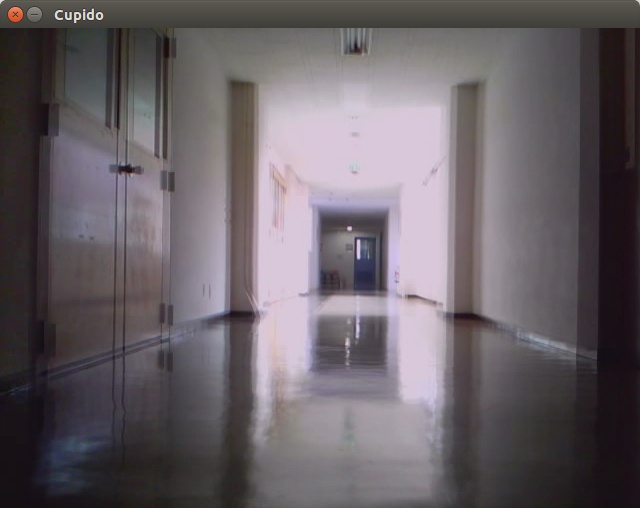
\includegraphics[width=0.4\columnwidth]{cupido_03.eps}}%
\hspace{0.1\columnwidth}%
\subfloat[Matching near features]{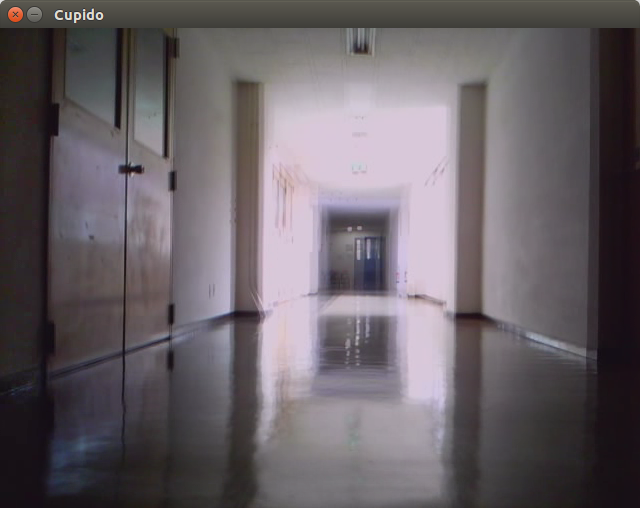
\includegraphics[width=0.4\columnwidth]{cupido_04.eps}}
\caption{Example screens from \textit{Cupido}, manual generator for image matching and shift ground truth data. Sampled teach and replay images are superimposed (a), and the user can skip back and forth over the teach stream, as well as shifting the current teach image horizontally, until a satisfactory match is found (b). Often, however, a decision must be made on whether to prioritize far (c) or near (d) features.}
\label{fig:cupido}
\end{figure}

\begin{figure}[t]
\subfloat[Indoors shift map]{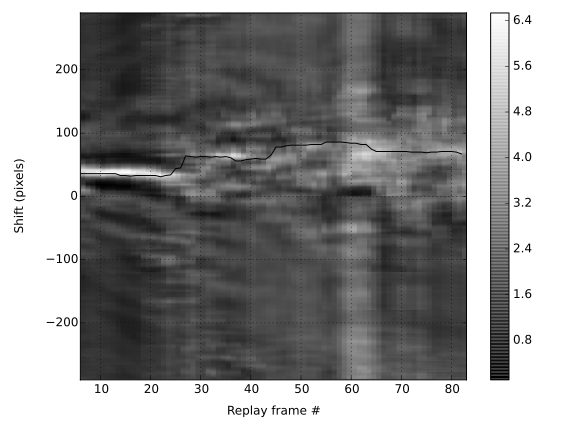
\includegraphics[width=\columnwidth]{shifts_indoors.pdf}}\\
\subfloat[Outdoors shift map]{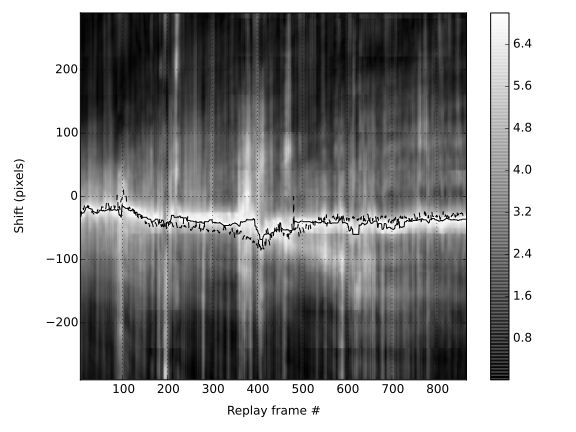
\includegraphics[width=\columnwidth]{shifts_outdoors.pdf}}
\caption{Shift maps for indoors (a) and outdoors (b) tests. Horizontal axis is replay step image by index number, and vertical axis is shift between teach and replay images -- positive values indicate left shift, and negative values, right. The contour map shows shift likelihood for each replay image across all possible shifts, with brighter pixels representing higher likelihood. A solid line indicates selected shifts across the replay sequence, and a dashed line, ground truth data computed manually. The indoors shift map (a) correctly indicates a left shift, consistent with the robot moving leftwards in the replay step relative to the teach step. The outdoors shift map (b) also correctly shows a right shift, consistent with the robot moving rightwards in the replay step relative to the teach step.}
\label{fig:shift_maps}
\end{figure}

\begin{figure}[t]
\subfloat[``Left turn'' shift map]{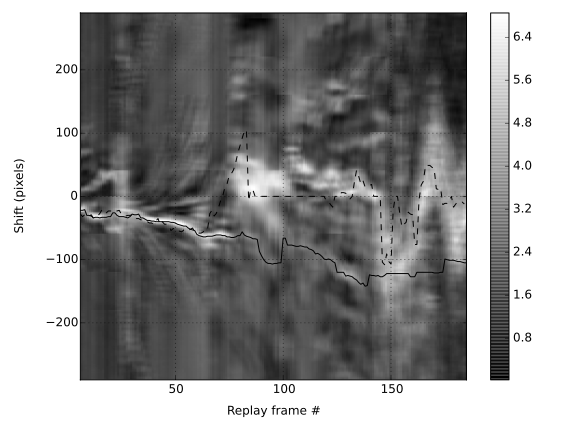
\includegraphics[width=\columnwidth]{shifts_turn_left.pdf}}\\
\subfloat[``Right turn'' shift map]{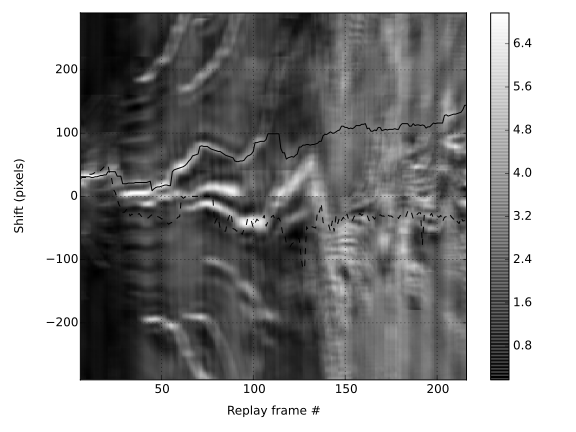
\includegraphics[width=\columnwidth]{shifts_turn_right.pdf}}
\caption{Shift maps for indoors tests over paths including either a left turn (between frames 1400 and 1600) (a) or right turn (between frames 300 and 700) (b). Horizontal axis is replay step image by index number, and vertical axis is shift between teach and replay images -- positive values indicate left shift, and negative values, right. The contour map shows shift likelihood for each replay image across all possible shifts, with brighter pixels representing higher likelihood. A solid line indicates selected shifts across the replay sequence, and a dashed line, ground truth data computed manually. On both cases shift maps loosely agree with ground truth shifts, however the shift selector algorithm is often unable to recognize such trends.}
\label{fig:shift_maps}
\end{figure}

A Yamabico robot with a front-mounted camera was set up to perform short trips over each environment, collecting video records (sampled at 20 FPS) along the way. The method described in the previous section was implemented on the Open Source C++ library \textbf{Cight}~\cite{HEL14c}, but unfortunately it was not possible to come up with a real-time implementation at this time. Therefore only off-line tests were performed. Method parameters were set to ($\alpha = 30, \beta = 80, n = 25, \tau = 25$). Initially, a single teach-replay session was recorded at each environment, with linear speed always set to $0.3m/s$.

The indoors environment was deserted when the teach step was recorded, but between $30s$ and $50s$ in the replay step video three people came from behind the robot, staying on the right side of the field of view as they walked away. The robot's initial pose in the replay step was turned $2^o$ to the left in relation to the teach step's, but otherwise both steps were recorded from the same start location. Figure~\ref{fig:environments}a-b show samples of these image sequences.

In the outdoors environment a pedestrian came from behind the robot during the teach step, staying on the left side of the visual field as he walked away from $20s$ to $40s$, but during the replay step there was no one in sight. The robot's initial pose in the replay step was turned $2^o$ to the right in relation to the teach step's, but otherwise both steps were recorded from the same start location. Figure~\ref{fig:environments}c-d show samples of these image sequences.

In order to evaluate the quality of image pairings and shift estimates, a tool for manually generating ground truth data was implemented. Dubbed \textit{Cupido}, the tool samples a record of the replay step at constant intervals, while the human user searches over the teach record for the frames (and horizontal shifts thereof) that produce the best matches. When a suitable match is found, indexes of the current teach and replay frames are recorded to a text file, along with the horizontal shift applied to the teach frame. Figure~\ref{fig:cupido} shows some example screens. Using the tool, it became clear that while it's sometimes possible to find near perfect matches (Fig.~\ref{fig:cupido}b), often the best match will be ambiguous: perfectly aligning teach and replay images across far features will leave near features mismatched (Fig.~\ref{fig:cupido}c), and vice versa (Fig.~\ref{fig:cupido}d). In the results presented below intermediary shifts (that would leave both near and far features ``almost matched'') were chosen whenever possible, but when differences were too large matching of far features was given priority. This may account for cases where ground truth values fall between pairs of strong estimates.

Figure~\ref{fig:shift_maps}a shows the shift map computed for the teach and replay trips recorded in the indoors environment, while Fig.~\ref{fig:shift_maps}b shows the shift maps between the outdoors teach and replay trips. The horizontal axis represent replay frames by index number, and the vertical axis, shift between teach and replay images -- positive values indicate left shift, and negative values, right. The contour map shows shift likelihood for each replay image across all possible shifts, with brighter pixels representing higher likelihood. A solid line indicates selected shifts across the replay sequence, and a dashed line, ground truth data computed manually. The indoors shift map (Fig.~\ref{fig:shift_maps}a) correctly indicates a left shift, consistent with the robot moving leftwards in the replay step relative to the teach step. The outdoors shift map (Fig.~\ref{fig:shift_maps}b) also correctly shows a right shift, consistent with the robot moving rightwards in the replay step relative to the teach step.

Additional tests were later recorded in the indoors environment to assess the method's performance during turning movements. Two extra trips were recorded, one containing a left turn at the later part of the trip (roughly between frames 1400 and 1600 of the replay trip) and another a right turn right at the beginning (between frames 300 and 700). In both cases shift maps loosely agree with ground truth shifts, however the shift selector algorithm is often unable to recognize such trends.

\section{Conclusion}

This article presented the \textit{Differential Visual Stream} (DiVS) image processing method. DiVS enabled quantitative comparison of image sequences of a landscape as captured by an approaching observer. This in turn can be employed to implement appearance-based navigation. Because the comparisons performed by DiVS are robust to many of the transitory differences between images of a same landscape, robust navigation can be achieved against changing environmental conditions.

A number of points still have to be addressed, however. The most pressing concern is the method's performance under actual autonomous navigation, a scenario that hasn't yet been explored due to the time shift estimates take to be computed (currently in the scale of seconds for every couple frames). Poor shift selection, especially over curved paths, is also of concern. Finally the effect of moving elements on shift estimation is still poorly understood.

Further research on ways to characterize an image sequence, extracting information useful for making inferences on robot movement, could provide important contributions towards solving some of those problems. For example, if it was possible to distinguish between ``straight'' and ``turning'' movements by observing a teach step stream, this information could be used to better inform robot steering during the replay step, even if shift estimation was poor.

\footnotesize

\bibliographystyle{IEEEtran}
\bibliography{references}

\normalsize

\end{document}
